% Options for packages loaded elsewhere
\PassOptionsToPackage{unicode}{hyperref}
\PassOptionsToPackage{hyphens}{url}
%
\documentclass[
]{book}
\usepackage{amsmath,amssymb}
\usepackage{lmodern}
\usepackage{iftex}
\ifPDFTeX
  \usepackage[T1]{fontenc}
  \usepackage[utf8]{inputenc}
  \usepackage{textcomp} % provide euro and other symbols
\else % if luatex or xetex
  \usepackage{unicode-math}
  \defaultfontfeatures{Scale=MatchLowercase}
  \defaultfontfeatures[\rmfamily]{Ligatures=TeX,Scale=1}
\fi
% Use upquote if available, for straight quotes in verbatim environments
\IfFileExists{upquote.sty}{\usepackage{upquote}}{}
\IfFileExists{microtype.sty}{% use microtype if available
  \usepackage[]{microtype}
  \UseMicrotypeSet[protrusion]{basicmath} % disable protrusion for tt fonts
}{}
\makeatletter
\@ifundefined{KOMAClassName}{% if non-KOMA class
  \IfFileExists{parskip.sty}{%
    \usepackage{parskip}
  }{% else
    \setlength{\parindent}{0pt}
    \setlength{\parskip}{6pt plus 2pt minus 1pt}}
}{% if KOMA class
  \KOMAoptions{parskip=half}}
\makeatother
\usepackage{xcolor}
\usepackage{color}
\usepackage{fancyvrb}
\newcommand{\VerbBar}{|}
\newcommand{\VERB}{\Verb[commandchars=\\\{\}]}
\DefineVerbatimEnvironment{Highlighting}{Verbatim}{commandchars=\\\{\}}
% Add ',fontsize=\small' for more characters per line
\usepackage{framed}
\definecolor{shadecolor}{RGB}{248,248,248}
\newenvironment{Shaded}{\begin{snugshade}}{\end{snugshade}}
\newcommand{\AlertTok}[1]{\textcolor[rgb]{0.94,0.16,0.16}{#1}}
\newcommand{\AnnotationTok}[1]{\textcolor[rgb]{0.56,0.35,0.01}{\textbf{\textit{#1}}}}
\newcommand{\AttributeTok}[1]{\textcolor[rgb]{0.77,0.63,0.00}{#1}}
\newcommand{\BaseNTok}[1]{\textcolor[rgb]{0.00,0.00,0.81}{#1}}
\newcommand{\BuiltInTok}[1]{#1}
\newcommand{\CharTok}[1]{\textcolor[rgb]{0.31,0.60,0.02}{#1}}
\newcommand{\CommentTok}[1]{\textcolor[rgb]{0.56,0.35,0.01}{\textit{#1}}}
\newcommand{\CommentVarTok}[1]{\textcolor[rgb]{0.56,0.35,0.01}{\textbf{\textit{#1}}}}
\newcommand{\ConstantTok}[1]{\textcolor[rgb]{0.00,0.00,0.00}{#1}}
\newcommand{\ControlFlowTok}[1]{\textcolor[rgb]{0.13,0.29,0.53}{\textbf{#1}}}
\newcommand{\DataTypeTok}[1]{\textcolor[rgb]{0.13,0.29,0.53}{#1}}
\newcommand{\DecValTok}[1]{\textcolor[rgb]{0.00,0.00,0.81}{#1}}
\newcommand{\DocumentationTok}[1]{\textcolor[rgb]{0.56,0.35,0.01}{\textbf{\textit{#1}}}}
\newcommand{\ErrorTok}[1]{\textcolor[rgb]{0.64,0.00,0.00}{\textbf{#1}}}
\newcommand{\ExtensionTok}[1]{#1}
\newcommand{\FloatTok}[1]{\textcolor[rgb]{0.00,0.00,0.81}{#1}}
\newcommand{\FunctionTok}[1]{\textcolor[rgb]{0.00,0.00,0.00}{#1}}
\newcommand{\ImportTok}[1]{#1}
\newcommand{\InformationTok}[1]{\textcolor[rgb]{0.56,0.35,0.01}{\textbf{\textit{#1}}}}
\newcommand{\KeywordTok}[1]{\textcolor[rgb]{0.13,0.29,0.53}{\textbf{#1}}}
\newcommand{\NormalTok}[1]{#1}
\newcommand{\OperatorTok}[1]{\textcolor[rgb]{0.81,0.36,0.00}{\textbf{#1}}}
\newcommand{\OtherTok}[1]{\textcolor[rgb]{0.56,0.35,0.01}{#1}}
\newcommand{\PreprocessorTok}[1]{\textcolor[rgb]{0.56,0.35,0.01}{\textit{#1}}}
\newcommand{\RegionMarkerTok}[1]{#1}
\newcommand{\SpecialCharTok}[1]{\textcolor[rgb]{0.00,0.00,0.00}{#1}}
\newcommand{\SpecialStringTok}[1]{\textcolor[rgb]{0.31,0.60,0.02}{#1}}
\newcommand{\StringTok}[1]{\textcolor[rgb]{0.31,0.60,0.02}{#1}}
\newcommand{\VariableTok}[1]{\textcolor[rgb]{0.00,0.00,0.00}{#1}}
\newcommand{\VerbatimStringTok}[1]{\textcolor[rgb]{0.31,0.60,0.02}{#1}}
\newcommand{\WarningTok}[1]{\textcolor[rgb]{0.56,0.35,0.01}{\textbf{\textit{#1}}}}
\usepackage{longtable,booktabs,array}
\usepackage{calc} % for calculating minipage widths
% Correct order of tables after \paragraph or \subparagraph
\usepackage{etoolbox}
\makeatletter
\patchcmd\longtable{\par}{\if@noskipsec\mbox{}\fi\par}{}{}
\makeatother
% Allow footnotes in longtable head/foot
\IfFileExists{footnotehyper.sty}{\usepackage{footnotehyper}}{\usepackage{footnote}}
\makesavenoteenv{longtable}
\usepackage{graphicx}
\makeatletter
\def\maxwidth{\ifdim\Gin@nat@width>\linewidth\linewidth\else\Gin@nat@width\fi}
\def\maxheight{\ifdim\Gin@nat@height>\textheight\textheight\else\Gin@nat@height\fi}
\makeatother
% Scale images if necessary, so that they will not overflow the page
% margins by default, and it is still possible to overwrite the defaults
% using explicit options in \includegraphics[width, height, ...]{}
\setkeys{Gin}{width=\maxwidth,height=\maxheight,keepaspectratio}
% Set default figure placement to htbp
\makeatletter
\def\fps@figure{htbp}
\makeatother
\setlength{\emergencystretch}{3em} % prevent overfull lines
\providecommand{\tightlist}{%
  \setlength{\itemsep}{0pt}\setlength{\parskip}{0pt}}
\setcounter{secnumdepth}{5}
\usepackage{booktabs}
\AtBeginDocument{\renewcommand{\chaptername}{S.}}
\usepackage{booktabs}
\usepackage{longtable}
\usepackage{array}
\usepackage{multirow}
\usepackage{wrapfig}
\usepackage{float}
\usepackage{colortbl}
\usepackage{pdflscape}
\usepackage{tabu}
\usepackage{threeparttable}
\usepackage{threeparttablex}
\usepackage[normalem]{ulem}
\usepackage{makecell}
\usepackage{xcolor}
\ifLuaTeX
  \usepackage{selnolig}  % disable illegal ligatures
\fi
\usepackage[]{natbib}
\bibliographystyle{apalike}
\IfFileExists{bookmark.sty}{\usepackage{bookmark}}{\usepackage{hyperref}}
\IfFileExists{xurl.sty}{\usepackage{xurl}}{} % add URL line breaks if available
\urlstyle{same} % disable monospaced font for URLs
\hypersetup{
  pdftitle={SPARTIN Supplementary material},
  pdfauthor={Nate Osher},
  hidelinks,
  pdfcreator={LaTeX via pandoc}}

\title{SPARTIN Supplementary material}
\author{Nate Osher}
\date{}

\begin{document}
\maketitle

{
\setcounter{tocdepth}{1}
\tableofcontents
}
\newcommand{\vb}[1]{\textcolor{blue}{\textsf{#1}}}
\newcommand{\no}[1]{\textcolor{red}{\textsf{[#1]}}}
\newcommand{\jk}[1]{\textcolor{violet}{\textsf{[JK: #1]}}}
\newcommand{\bs}[1]{{\boldsymbol{#1}}}
\newcommand{\bm}[1]{{\mathbf{#1}}}

\hypertarget{preface}{%
\chapter{Preface}\label{preface}}

The purpose of this document is to serve as a ``living'' supplement to the
first paper on the SPARTYN pipeline. While the paper itself will be
static upon publication, this document will serve as both an ongoing
supplement as well as a central location to give updated, detailed
information on the pipeline and methods.

If you have a question that is not adequately addressed in this
supplement, please email oshern (at) umich.edu.

\hypertarget{model-fitting}{%
\chapter{Model Fitting}\label{model-fitting}}

Given a quadrature \({\mathbf{u}}\) on \(A\) with corresponding weights \({\mathbf{w}}\), the pseduolikelihood function (equation (3) in the main paper) can be approximated by

\begin{equation}
\label{eqn:PL_approx}
PL(\theta | {\mathbf{x}}) \approx
\prod_{x_i \in {\mathbf{x}}} \lambda(x_i | \theta, {\mathbf{x}}) \exp(-\sum_{u_j \in {\mathbf{u}}} \lambda(u_j | \theta, {\mathbf{x}}) w_j) \tag{S1}
\end{equation}

The density of the selected quadrature \({\mathbf{u}}\) on \(A\) is chosen to balance the accuracy of the approximation against the computational load that larger quadratures impose.

Using this approximation of the pseudolikelihood function in place of the more standard likelihood function, Bayesian analysis can proceed in the style of \citet{King12} by simply assigning priors to the parameters of interest and using techniques to sample from non-closed form posterior likelihoods. We assigned non-informative normal priors with mean 0 and variance \(10^6\) to \(\log(\gamma_{12})\), \(\log(\beta_1)\), and \(\log(\beta_2)\). In all analysis presented in the main paper the quadrature and weights used to estimate the integral in the pseudolikelihood function was generated by the spatstat package (\citet{BT05}). Samples from the posterior were taken using JAGS via the R2jags package (\citet{Su15}).

In order to use JAGS to fit the model, the so-called ``Poisson zero trick'' as described in \citet{Kruschke14}. This allows for the fitting of a model with an arbitrary likelihood (or pseudolikelihood) function. The zero trick works by explicitly specifying the log-likelihood function of the model to be fit for each observation, and treating the resulting log-likelihood as the rate parameter of a Poisson distribution. Note that because the log-likelihood function can be negative, a constant value may have to be added in order to ensure the resulting value is strictly positive, since the rate parameter of a Poisson distribution must be strictly positive. But if the same value is used for all observations in a single model fitting across iterations, this is equivalent to multiplying the likelihood by a constant, which does not affect the inference. A vector of zeros is passed to JAGS, and each zero is said to be observed from a Poisson distribution with rate parameter specified by the modified log-likelihood function evaluated for that observation. By definition of the probability mass function of the Poisson distribution, the resulting likelihood is the target likelihood for each observation. An analogous trick using the Bernoulli distribution and a vector of ones can be used as well- see \citet{Kruschke14} for details. Briefly, denoting the number of observed points \(n_o\), the number of quadrature points \(n_q\), and \(n_o + n_q = N\), the underlying MCMC algorithm is as follows

\begin{center}\rule{0.5\linewidth}{0.5pt}\end{center}

\textbf{Algorithm 1S}: Bayesian Strauss Model Fitting

\begin{center}\rule{0.5\linewidth}{0.5pt}\end{center}

\textbf{Input:} Type vector \(t_1, \dots, t_N\), weight vector \(w_1, \dots, w_N\), and neighbor counts \(c_1, \dots, c_N\)

\textbf{For} \(i = 1, \dots, n\_iter\) \textbf{do}:\\
\textbar{} \textbf{For} \(\theta = \beta_1, \beta_2, \gamma_{12}\) \textbf{do}:\\
\textbar{} \textbar{} Propose \(\theta^*\)\\
\textbar{} \textbar{} Evaluate PL(\theta\^{}* \textbar{} \cdot )\\
\textbar{} \textbar{} Set \(\theta^{(i)} = \theta^*\) with probability \(min(\frac{PL(\theta^*)}{PL(\theta)}, 1)\); otherwise, set \(\theta^{(i)} = \theta\)\\
\textbar{} \textbf{End For}\\
\textbf{End For}

\textbf{Return:} \(\beta_1^{(1)}, \dots, \beta_1^{(n\_iter)}\), \(\beta_2^{(1)}, \dots, \beta_2^{(n\_iter)}\), \(\gamma_{12}^{(1)}, \dots, \gamma_{12}^{(n\_iter)}\)

\begin{center}\rule{0.5\linewidth}{0.5pt}\end{center}

Results were checked against both frequentist model fittings from the spatstat \texttt{ppm}/\texttt{hierstrauss} functions as well as STAN model fittings (\citet{Carpenter17}) and yielded virtually indistinguishable results in both cases. Despite STAN sampling more quickly than JAGS, JAGS still outperformed STAN due to its somewhat shorter time in setting up the model for sampling.

\hypertarget{biopsy-partition}{%
\chapter{Biopsy Partition}\label{biopsy-partition}}

In order to partition a given biopsy into non-overlapping sub-regions, we began with the smallest bounding rectangular window that contained all cells. We then applied an intensity thresholding algorithm in order to find the smallest possible window that still contained virtually all cells. This was accomplished using the \texttt{density.ppp} function from the \texttt{spatstat} package (\citet{BT05}). The bounding rectangular window was broken up into small (15\(\mu m\) \(\times\) 15\(\mu m\)) pixels, the intensity of which was estimated as a function of the number of points per square unit of area of the pixel. These values were also ``smoothed'' between pixels according to a pre-selected bandwidth of 25\(\mu m\) chosen through experimentation. The final window was constructed by combining all pixels that were above a certain intensity into a window. The ``pixel'' size, smoothing bandwidth, and intensity threshold collectively determined the final window, and the same settings (15\(\mu m^2\) pixel size and \(25\mu m\) smoothing bandwidth) were applied across all biopsies.

\hypertarget{cell-classification-model}{%
\chapter{Cell Classification Model}\label{cell-classification-model}}

\hypertarget{whole-slide-image-wsi-retrieval-and-obtaining-training-labels}{%
\section{Whole-Slide Image (WSI) Retrieval and Obtaining Training Labels}\label{whole-slide-image-wsi-retrieval-and-obtaining-training-labels}}

WSI from 20 different patients were used as our primary training and testing data. The images were imported from The Cancer Genome Atlas (TCGA) Genomic Data Commons Data Portal, which is a repository of validated datasets from various National Cancer Institute Programs. Also known as the gigapixel pathology image, one image slide contained two tissue smears stained with hematoxylin and eosin, imported in a vendor specific format. The imported image for classification is scanned at the `high' magnification level in a microscope of 40X. The pixel size for images was approximately 0.25 microns per pixel. Manual marking of a minimum of ten samples from each of the classes i.e., Tumors, Immune, Macrophage, and other cell was performed by a pathologist on all slides. Care was taken to ensure that the samples were as diverse as possible, to account for all possible morphologies of the same cell type across all cases. In total, 1250 annotations were made in all the images, with each annotated cell labelled by a pathologist. The reasons for the comparatively smaller labelled dataset available lie in the large size of the slide, and pathologist availability; the large size makes parsing through difficult and explains the diversity of labelled structures in each image.

\hypertarget{whole-slide-image-wsi-nucleus-segmentation}{%
\section{Whole-Slide Image (WSI) Nucleus Segmentation}\label{whole-slide-image-wsi-nucleus-segmentation}}

Before nuclear segmentation and extraction can be performed on the WSIs, certain pre-processing steps are carried out to ensure staining uniformity across images. A representative and generalizable stain vector estimation for each of the stains being used in the image is estimated, to normalize the staining intensities across all the images. In our application, vectors from hematoxylin, eosin and residual stains were estimated from a standard image, selected by the clinician. These vectors are then applied across all images to keep the stain detection parameters uniform across the dataset (\citet{Bankhead18}).

Due to the variations in staining procedures across the dataset, it is difficult to accurately isolate whole cells on the slide, as the cytoplasmic boundaries are not well-defined due to lack of membrane staining. As heterogeneity in nuclear morphology has been shown to be a good discriminator, only the nucleus is segmented out of each cell in every image for classification purposes, using Qupath (\citet{Yuan12}). Watershed segmentation is used to obtain separated and contoured nuclei from the hematoxylin color channel of the whole slide image, in a patch-based manner (\citet{Bankhead18}). The separate hematoxylin channel is obtained by performing color deconvolution to separate out the stains used in the slide (\citet{Ruifrok01}). It was observed that an average of 200,000 cells were segmented out per image, and morphological and intensity features such as spatial location, eccentricity, circularity, and stain intensities were computed. All pertinent image analysis and nuclear segmentation was performed using Qupath, an open-sourced software platform that can be used for a range of pathological image analysis applications (\citet{Bankhead17}).

\begin{tabular}{l|l|l|l|l|l}
\hline
Class & Tumor (1) & Immune (2) & Other Cells (3) & Macrophage (4) & Total Cells\\
\hline
Number of Labels & 288 & 349 & 252 & 361 & 1250\\
\hline
\multicolumn{6}{l}{\textsuperscript{} Table 4.2: Cell type composition of training dataset.}\\
\end{tabular}

A Random Forest model is a type of ensemble learning method, where the weak predictive power of multiple decision trees is aggregated to produce an accurate result \citet{Breiman01}. Our four-class classifier model was developed with a pathologist labelled dataset of 1250 morphologically diverse cells, each belonging to Tumor, Immune, Macrophage, or other cells (including cell types such as stromal cells). 5-fold cross-validation was used to assess model accuracy and the receiver operator characteristic curve AUC for each class, with proportional representation of all 4 classes ensured. After adjusting for multiple parameters, including the number of decision trees, the accuracy was obtained in the range of 87-91\%.

This step allowed for a preparation of a dataset for each cell with its spatial location using global coordinates and class of the cell, which is then used for further downstream analysis. The training, testing, and classification of cells from the WSIs was performed on MATLAB version 2017A.

\hypertarget{genomic-associations}{%
\chapter{Genomic Associations}\label{genomic-associations}}

\hypertarget{association-with-expression-of-significantly-mutated-genes}{%
\section{Association with expression of significantly mutated genes}\label{association-with-expression-of-significantly-mutated-genes}}

In addition to associations with survival, we investigated the
association between our measurement and gene expression. Gene
expression data was acquired for all 335 patients in
our sample using TCGA Assembler (\citet{Zhu14}). Additionally,
42 significantly mutated genes (SMGs) of interest were identified
using previous work investigating the genomic differences in
SKCM (\citet{Akbani15}).

Of the 335 patients in our sample, 330 had gene expression data
for all genes of interest, while 95 were missing data for all
genes of interest. We examined the marginal association between
the normalized gene expression data for the 330 patients with
complete data and average logit CTIP values. Marginal association
was assessed via univariate simple linear regression, carried out
separately for each gene. The Wald statistic of the coefficient
corresponding to gene expression was used to produce a \(p\)-value.
After correcting for multiple testing using a Bonferroni correction with \(\alpha = 0.05\), we found that LRRC37A3 was significantly positively associated with
average logit CTIP (\(p << 0.0001\)). See Table 5.2 below for the full list of genes, significance of associations, and directionality of associations.

\begin{tabular}{l|l|l}
\hline
Gene & P-value & Direction of Association\\
\hline
LRRC37A3 & 3.9e-05 * & Positive\\
\hline
B2M & 0.0012 & Negative\\
\hline
TP53 & 0.0019 & Positive\\
\hline
BRAF & 0.024 & Negative\\
\hline
RCAN2 & 0.027 & Positive\\
\hline
TMEM216 & 0.032 & Positive\\
\hline
ACD & 0.033 & Positive\\
\hline
PPIAL4G & 0.043 & Positive\\
\hline
TBC1D3B & 0.052 & Positive\\
\hline
FAM113B & 0.055 & Negative\\
\hline
COL9A2 & 0.057 & Positive\\
\hline
SIRPB1 & 0.064 & Negative\\
\hline
ZFX & 0.073 & Negative\\
\hline
RB1 & 0.087 & Negative\\
\hline
DDX3X & 0.1 & Negative\\
\hline
RQCD1 & 0.13 & Negative\\
\hline
CCDC28A & 0.14 & Negative\\
\hline
NDUFB9 & 0.15 & Positive\\
\hline
EMG1 & 0.15 & Positive\\
\hline
ITGA4 & 0.18 & Positive\\
\hline
OXA1L & 0.19 & Positive\\
\hline
CTNNB1 & 0.2 & Negative\\
\hline
STK19 & 0.27 & Positive\\
\hline
MAP2K1 & 0.28 & Negative\\
\hline
NRAS & 0.28 & Negative\\
\hline
GNAI2 & 0.32 & Positive\\
\hline
RAPGEF5 & 0.36 & Positive\\
\hline
NF1 & 0.37 & Negative\\
\hline
IDH1 & 0.37 & Negative\\
\hline
PTEN & 0.4 & Negative\\
\hline
ARID2 & 0.42 & Negative\\
\hline
RAC1 & 0.42 & Positive\\
\hline
CDKN2A & 0.56 & Positive\\
\hline
MRPS31 & 0.64 & Positive\\
\hline
MSR1 & 0.7 & Negative\\
\hline
WDR12 & 0.72 & Negative\\
\hline
NOTCH2NL & 0.83 & Positive\\
\hline
PPP6C & 0.85 & Positive\\
\hline
C3orf71 & 0.89 & Negative\\
\hline
RPS27 & 0.9 & Negative\\
\hline
FAM58A & 0.95 & Positive\\
\hline
KNSTRN & 0.98 & Positive\\
\hline
\multicolumn{3}{l}{\textsuperscript{} Table 5.2: Significantly mutated genes,}\\
\multicolumn{3}{l}{unadjusted p-values, and direction of}\\
\multicolumn{3}{l}{association with biopsy level average logit}\\
\multicolumn{3}{l}{CTIP. Asterisk indicates significance under}\\
\multicolumn{3}{l}{Bonferroni correction, alpha = 0.05.}\\
\end{tabular}

\hypertarget{association-with-expression-of-immune-genes}{%
\section{Association with expression of immune genes}\label{association-with-expression-of-immune-genes}}

We also assessed the association between CTIP and genes that are
associated with immune activity. \citet{Bhattacharya18} have collected and classified a list of 1,793 unique genes associated with various aspects of human immune activity. Of these, gene expression data was available for 1,305 genes across the same 330 patients used in the previous gene expression analysis. We assessed the univariate association between biopsy level mean logit CTIP and these genes using Spearman Correlation. The advantage of Spearman correlation as opposed to the more standard Pearson correlation is that the former does not assume a linear relationship between the underlying variables of interest. Such assumptions can be problematic, particularly when there is no strong reason a priori to believe the relationship between the two variables is of a particular form. However, like Pearson correlation Spearman correlation is defined to lie in \([-1,1]\), with each extreme indicating the same directionality and strength of association as Pearson Correlation. Finally, statistical significance of associations was calculated using the cor.test function of the R programming language (\citet{Rteam}). After applying a Bonferroni correction, we found that 28 genes were significantly associated with IP. For the complete list of genes, see Table 5.2 below.

\begin{figure}

{\centering 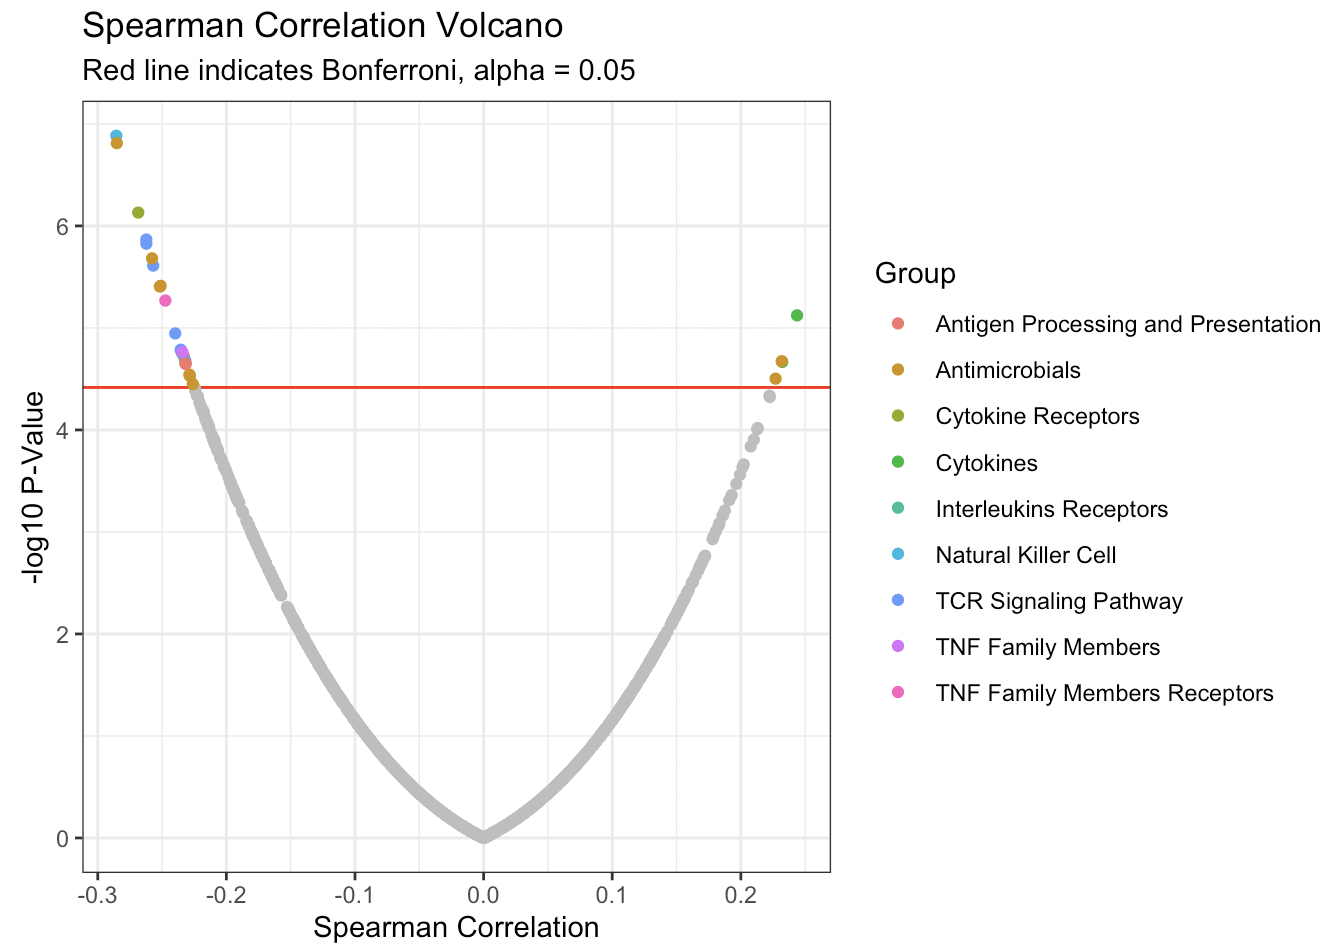
\includegraphics[width=1\linewidth]{Figures/IMMPORT Spearman} 

}

\caption{$-log_{10}$ p-values plotted against Spearman Correlation. Colors indicate Group as determined by IMMPORT; Red line indicates Bonferroni correction}\label{fig:04}
\end{figure}

\begin{tabular}{l|l|l|l}
\hline
Gene & Group & Spearman Correlation & P-Value\\
\hline
CD244 & Natural Killer Cell & -0.29 & << 0.0001\\
\hline
CTSS & Antimicrobials & -0.29 & << 0.0001\\
\hline
CCR8 & Cytokine Receptors & -0.27 & << 0.0001\\
\hline
CD3G & TCR Signaling Pathway & -0.26 & << 0.0001\\
\hline
PTPRC & TCR Signaling Pathway & -0.26 & << 0.0001\\
\hline
TLR8 & Antimicrobials & -0.26 & << 0.0001\\
\hline
ITK & TCR Signaling Pathway & -0.26 & << 0.0001\\
\hline
TLR3 & Antimicrobials & -0.25 & << 0.0001\\
\hline
STAT1 & Antimicrobials & -0.25 & << 0.0001\\
\hline
TNFRSF9 & TNF Family Members Receptors & -0.25 & << 0.0001\\
\hline
EREG & Cytokines & 0.24 & << 0.0001\\
\hline
LCK & TCR Signaling Pathway & -0.24 & < 0.0001\\
\hline
PIK3CG & TCR Signaling Pathway & -0.24 & < 0.0001\\
\hline
ERAP1 & Antigen Processing and Presentation & -0.24 & < 0.0001\\
\hline
TNFSF14 & TNF Family Members & -0.23 & < 0.0001\\
\hline
IL6R & Interleukins Receptors & -0.23 & < 0.0001\\
\hline
CIITA & Antigen Processing and Presentation & -0.23 & < 0.0001\\
\hline
ICOS & TCR Signaling Pathway & -0.23 & < 0.0001\\
\hline
DES & Antimicrobials & 0.23 & < 0.0001\\
\hline
APLN & Cytokines & 0.23 & < 0.0001\\
\hline
IFIH1 & Antimicrobials & -0.23 & < 0.0001\\
\hline
RFX5 & Antigen Processing and Presentation & -0.23 & < 0.0001\\
\hline
LYZ & Antimicrobials & -0.23 & < 0.0001\\
\hline
CXCR6 & Cytokine Receptors & -0.23 & < 0.0001\\
\hline
CRABP1 & Antimicrobials & 0.23 & < 0.0001\\
\hline
CYBB & Antimicrobials & -0.23 & < 0.0001\\
\hline
\multicolumn{4}{l}{\textsuperscript{} Table 5.2: IMMPORT Genes significantly associated with average}\\
\multicolumn{4}{l}{logit biopsy level CTIP after Bonferroni correction, alpha = 0.05.}\\
\end{tabular}

\hypertarget{association-with-deconvolution-data}{%
\chapter{Association with Deconvolution Data}\label{association-with-deconvolution-data}}

Using data from TIMER2.0 (\citet{TIMER20}), we examined the association between the prevalence of different types of immune cells and biopsy level mean logit CTIP. We ultimately decided to use the MCP-counter algorithm (\citet{Becht16}) based on the analysis of \citet{Sturm19}, since it was judged to be most effective in detecting the presence and prevalence of the most relevant types of immune cells. We investigated the association of the score of each type of immune cell estimated by MCP-counter with biopsy level mean logit CTIP using Spearman correlation. Significance was assessed using the standard test of statistical significance of Spearman correlation as implemented by the pspearman package.

After applying a Bonferroni correction (\(\alpha = 0.05\)), we found that six different immune cell scores as computed by MCP-counter were significantly negatively associated with biopsy level mean logit CTIP: CD8+ T cells, B cells, Monocytes, Macrophages, Myeloid Dendritic Cells, and Natural Killer cells. No cell types were significantly positively associated with biopsy level mean logit CTIP after the Bonferroni correction, though the magnitude of the positive association with Cancer Associated Fibroblasts (CAFs) is notable, and while not statistically significant still highly consistent with a truly positive underlying association between biopsy level CTIP and prevalence of CAFs.

\begin{figure}

{\centering 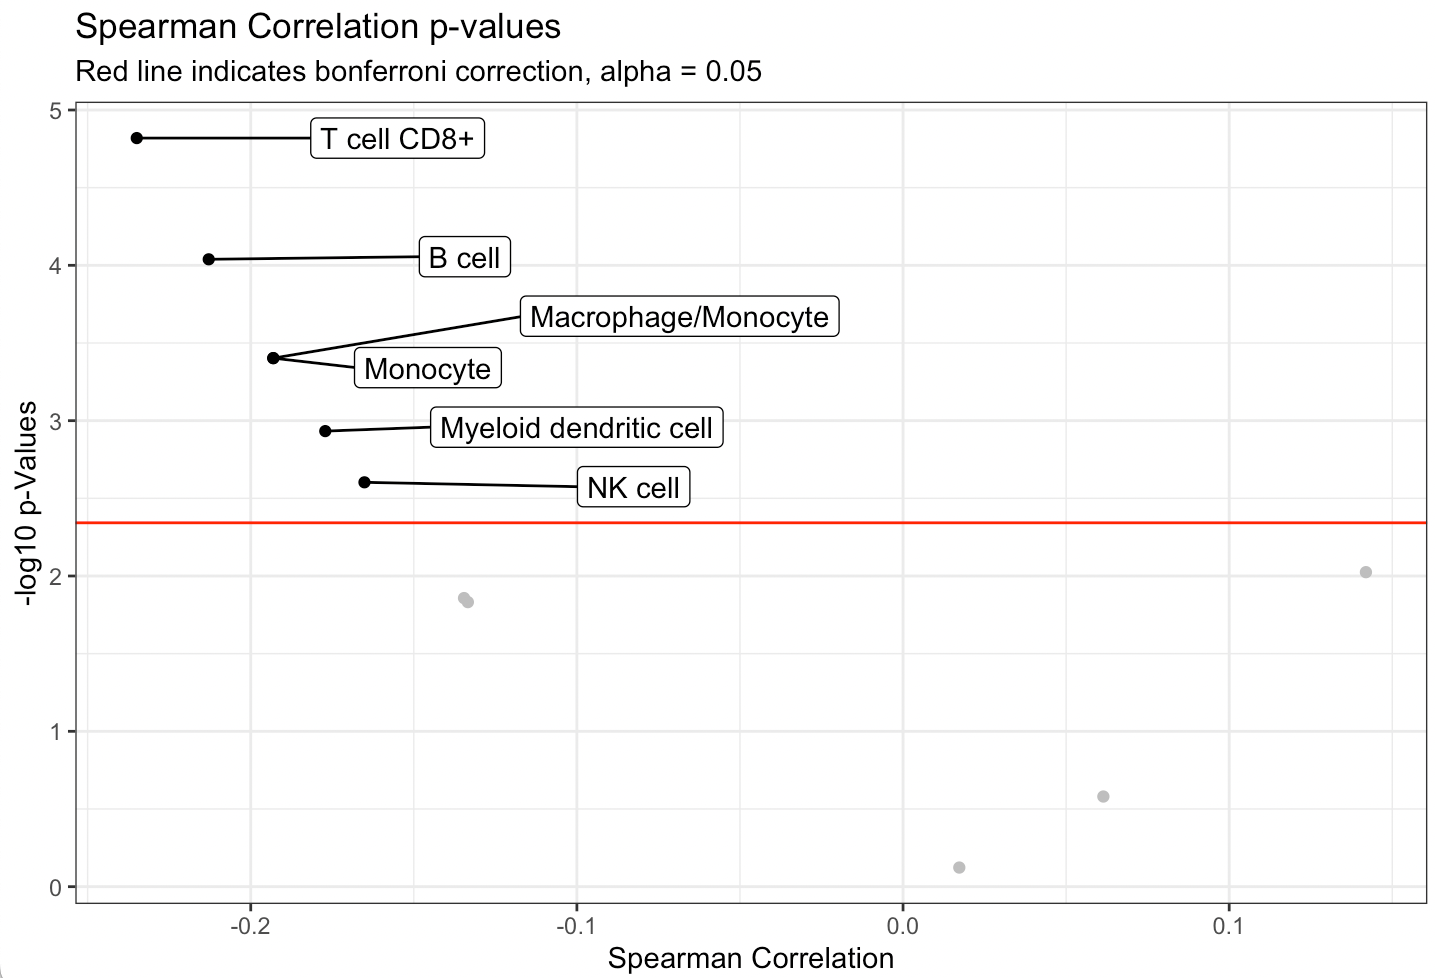
\includegraphics[width=1\linewidth]{Figures/MCP Spearman Volcano} 

}

\caption{Negative log-10 p-values plotted against Spearman Correlation. Colors indicate Group as determined by IMMPORT; Red line indicates Bonferroni correction, alpha = 0.05.}\label{fig:05}
\end{figure}

\begin{tabular}{l|r|r}
\hline
Cell Type & Spearman Correlation & P-Value\\
\hline
T cell & -0.1345989 & 0.0138744\\
\hline
T cell CD8+ & -0.2349456 & 0.0000152\\
\hline
cytotoxicity score & -0.1334298 & 0.0147288\\
\hline
NK cell & -0.1651353 & 0.0024940\\
\hline
B cell & -0.2128785 & 0.0000914\\
\hline
Monocyte & -0.1930875 & 0.0003958\\
\hline
Macrophage/Monocyte & -0.1930875 & 0.0003958\\
\hline
Myeloid dendritic cell & -0.1771510 & 0.0011674\\
\hline
Neutrophil & 0.0172481 & 0.7533506\\
\hline
Endothelial cell & 0.0614183 & 0.2628597\\
\hline
Cancer associated fibroblast & 0.1419220 & 0.0094486\\
\hline
\multicolumn{3}{l}{\textsuperscript{} Table 6.1: IMMPORT Genes significantly associated with}\\
\multicolumn{3}{l}{average logit biopsy level CTIP after Bonferroni}\\
\multicolumn{3}{l}{correction, alpha = 0.05.}\\
\end{tabular}

\hypertarget{spartin-r-package}{%
\chapter{SPARTIN R package}\label{spartin-r-package}}

This is a brief tutorial on the usage of the SPARTIN R package. It is also available as a vignette in the package itself.

\begin{Shaded}
\begin{Highlighting}[]
\FunctionTok{library}\NormalTok{(spatstat)}
\FunctionTok{library}\NormalTok{(SPARTIN)}
\FunctionTok{library}\NormalTok{(purrr)}
\FunctionTok{set.seed}\NormalTok{(}\DecValTok{10000}\NormalTok{)}
\end{Highlighting}
\end{Shaded}

The following two functions are purely for visualization. They aren't technically part of the package (yet), but you may find them useful if you decide to use this package. Regardless, we'll be using them for this vignette.

\begin{Shaded}
\begin{Highlighting}[]
\NormalTok{CustomHeatmap }\OtherTok{=}\NormalTok{ CH }\OtherTok{=} \ControlFlowTok{function}\NormalTok{(m, }\AttributeTok{t=}\StringTok{""}\NormalTok{, }\AttributeTok{min.v =} \ConstantTok{NA}\NormalTok{, }\AttributeTok{max.v =} \ConstantTok{NA}\NormalTok{)\{}
\NormalTok{  plot.tib }\OtherTok{=} \FunctionTok{tibble}\NormalTok{(}\AttributeTok{r =} \FunctionTok{numeric}\NormalTok{(}\DecValTok{0}\NormalTok{), }\AttributeTok{c =} \FunctionTok{numeric}\NormalTok{(}\DecValTok{0}\NormalTok{), }\AttributeTok{val =} \FunctionTok{numeric}\NormalTok{(}\DecValTok{0}\NormalTok{))}
  \ControlFlowTok{for}\NormalTok{(i }\ControlFlowTok{in} \DecValTok{1}\SpecialCharTok{:}\FunctionTok{nrow}\NormalTok{(m))\{}
\NormalTok{    plot.tib }\OtherTok{=} \FunctionTok{bind\_rows}\NormalTok{(plot.tib, }\FunctionTok{tibble}\NormalTok{(}
      \AttributeTok{r =} \FunctionTok{rep}\NormalTok{(i, }\FunctionTok{ncol}\NormalTok{(m)),}
      \AttributeTok{c =} \DecValTok{1}\SpecialCharTok{:}\FunctionTok{ncol}\NormalTok{(m),}
      \AttributeTok{val =} \FunctionTok{as.numeric}\NormalTok{(m[i,])))}
\NormalTok{  \}}
  
\NormalTok{  plot.tib}\SpecialCharTok{$}\NormalTok{c }\OtherTok{=} \FunctionTok{as.factor}\NormalTok{(plot.tib}\SpecialCharTok{$}\NormalTok{c)}

  \ControlFlowTok{if}\NormalTok{(}\FunctionTok{is.na}\NormalTok{(min.v) }\SpecialCharTok{||} \FunctionTok{is.na}\NormalTok{(max.v))\{}
\NormalTok{    min.v }\OtherTok{=} \FunctionTok{min}\NormalTok{(plot.tib}\SpecialCharTok{$}\NormalTok{val, }\AttributeTok{na.rm =}\NormalTok{ T)}
\NormalTok{    max.v }\OtherTok{=} \FunctionTok{max}\NormalTok{(plot.tib}\SpecialCharTok{$}\NormalTok{val, }\AttributeTok{na.rm =}\NormalTok{ T)}
\NormalTok{  \}}
\NormalTok{  cols }\OtherTok{=} \FunctionTok{colorRampPalette}\NormalTok{(}\FunctionTok{c}\NormalTok{(}\StringTok{"\#0a0722"}\NormalTok{, }\StringTok{"\#3d0965"}\NormalTok{, }\StringTok{"\#721a6e"}\NormalTok{, }\StringTok{"\#a52c60"}\NormalTok{, }\StringTok{"\#d44842"}\NormalTok{,}
                            \StringTok{"\#f37819"}\NormalTok{, }\StringTok{"\#fcb216"}\NormalTok{))(}\DecValTok{7}\NormalTok{) }\CommentTok{\#, "\#f1f179"))(8)}

  \FunctionTok{ggplot}\NormalTok{(plot.tib) }\SpecialCharTok{+}
    \FunctionTok{geom\_tile}\NormalTok{(}\AttributeTok{mapping =} \FunctionTok{aes}\NormalTok{(}\AttributeTok{x =}\NormalTok{ c, }\AttributeTok{y =} \FunctionTok{reorder}\NormalTok{(r, }\SpecialCharTok{{-}}\NormalTok{r), }\AttributeTok{fill =}\NormalTok{ val)) }\SpecialCharTok{+}
    \FunctionTok{labs}\NormalTok{(}\AttributeTok{fill =} \StringTok{""}\NormalTok{) }\SpecialCharTok{+}
    \FunctionTok{ggtitle}\NormalTok{(t) }\SpecialCharTok{+}
    \FunctionTok{scale\_fill\_gradientn}\NormalTok{(}\AttributeTok{colors =}\NormalTok{ cols,}
                         \AttributeTok{limits =} \FunctionTok{c}\NormalTok{(min.v, max.v),}
                         \CommentTok{\# breaks = seq(min.v, max.v, 2),}
                         \AttributeTok{na.value =} \StringTok{\textquotesingle{}white\textquotesingle{}}\NormalTok{) }\SpecialCharTok{+}
    \FunctionTok{theme}\NormalTok{(}\AttributeTok{axis.title.y=}\FunctionTok{element\_blank}\NormalTok{(),}
          \AttributeTok{axis.text.y=}\FunctionTok{element\_blank}\NormalTok{(),}
          \AttributeTok{axis.ticks.y=}\FunctionTok{element\_blank}\NormalTok{(),}
          \AttributeTok{axis.title.x=}\FunctionTok{element\_blank}\NormalTok{(),}
          \AttributeTok{axis.text.x=}\FunctionTok{element\_blank}\NormalTok{(),}
          \AttributeTok{axis.ticks.x=}\FunctionTok{element\_blank}\NormalTok{(),}
          \AttributeTok{panel.background =} \FunctionTok{element\_rect}\NormalTok{(}\AttributeTok{fill =} \StringTok{"white"}\NormalTok{,}
                                          \AttributeTok{colour =} \StringTok{"black"}\NormalTok{),}
          \AttributeTok{panel.border =} \FunctionTok{element\_rect}\NormalTok{(}\AttributeTok{linetype =} \StringTok{"solid"}\NormalTok{, }\AttributeTok{fill =} \ConstantTok{NA}\NormalTok{))}
\NormalTok{\}}

\CommentTok{\# Visualize PPP}
\NormalTok{vis }\OtherTok{=} \ControlFlowTok{function}\NormalTok{(p, }\AttributeTok{t=}\StringTok{""}\NormalTok{, }\AttributeTok{suppWarn =}\NormalTok{ F)\{}
  \ControlFlowTok{if}\NormalTok{(suppWarn)\{}
    \FunctionTok{suppressWarnings}\NormalTok{(}
      \FunctionTok{plot}\NormalTok{(p, }\AttributeTok{cols =} \FunctionTok{c}\NormalTok{(}\StringTok{"black"}\NormalTok{, }\StringTok{"red"}\NormalTok{),}
           \AttributeTok{shape =} \FunctionTok{c}\NormalTok{(}\StringTok{"circles"}\NormalTok{, }\StringTok{"circles"}\NormalTok{),}
           \AttributeTok{size =} \DecValTok{6}\NormalTok{,}
           \AttributeTok{main =}\NormalTok{ t)}
\NormalTok{    )}
\NormalTok{  \}}\ControlFlowTok{else}\NormalTok{\{}
    \FunctionTok{plot}\NormalTok{(p, }\AttributeTok{cols =} \FunctionTok{c}\NormalTok{(}\StringTok{"black"}\NormalTok{, }\StringTok{"red"}\NormalTok{),}
         \AttributeTok{shape =} \FunctionTok{c}\NormalTok{(}\StringTok{"circles"}\NormalTok{, }\StringTok{"circles"}\NormalTok{),}
         \AttributeTok{size =} \DecValTok{6}\NormalTok{,}
         \AttributeTok{main =}\NormalTok{ t)}
\NormalTok{  \}}
\NormalTok{\}}
\end{Highlighting}
\end{Shaded}

\hypertarget{simulation-and-model-fitting}{%
\section{Simulation and Model Fitting}\label{simulation-and-model-fitting}}

First, we'll simulate some data.

\begin{Shaded}
\begin{Highlighting}[]
\NormalTok{ex\_ppp }\OtherTok{=} \FunctionTok{SimulateData}\NormalTok{(}\AttributeTok{n1 =} \DecValTok{100}\NormalTok{, }\AttributeTok{n2 =} \DecValTok{40}\NormalTok{, }\AttributeTok{phi =} \FloatTok{0.3}\NormalTok{,}
                      \AttributeTok{winX =} \DecValTok{300}\NormalTok{, }\AttributeTok{winY =} \DecValTok{300}\NormalTok{, }\AttributeTok{r =} \DecValTok{30}\NormalTok{)}
\end{Highlighting}
\end{Shaded}

Breaking down this function call:

\begin{itemize}
\tightlist
\item
  \texttt{n1} specifies the number of points of type 1
\item
  \texttt{n2} specifies the number of points of type 2
\item
  \texttt{phi} specifies the interaction between the points, -1 being the most negative (points of different types tend to ``avoid'' each other) and 1 being the most positive (points of different types tend to be close together)
\item
  \texttt{winX} specifies the horizontal width of the window of simulation
\item
  \texttt{winY} specifies the vertical height of the window of simulation
\item
  \texttt{r} specifies the radius of interaction
\end{itemize}

Next, we'll fit a Frequentist version of the model using the \texttt{FitHSFreq} function. The ``HS'' stands for ``Hierarchical Strauss,'' the variant of the model that we'll be using. This is essentially a wrapper around the \texttt{spatstat} function \texttt{ppm} with certain parameters, since the SPARTIN pipeline uses a special case of the Hierarchical Strauss model. Below, I pass the point process we simulated, and specify that the radius of interaction is 30 units, and that the quadrature used in the fitting should have 3 units of space between each point. As always, there is a tradeoff here: the larger the quadrature (and thus the smaller that \texttt{quad.spacing} parameter), the more accurate the fitting will be. However, it will also be more computationally expensive. On the other hand, a small quadrature may lead to quicker fittings, but may also be less accurate. Unfortunately, there isn't a one size fits all solution to this across all use cases. Some situations call for larger quadratures and more precise estimation, while for others a rough approximation will probably be fine.

\begin{Shaded}
\begin{Highlighting}[]
\NormalTok{ex\_freq }\OtherTok{=} \FunctionTok{FitHSFreq}\NormalTok{(ex\_ppp, }\AttributeTok{r =} \DecValTok{30}\NormalTok{, }\AttributeTok{quad.spacing =} \DecValTok{3}\NormalTok{)}
\FunctionTok{coef}\NormalTok{(}\FunctionTok{summary}\NormalTok{(ex\_freq))}
\end{Highlighting}
\end{Shaded}

\begin{verbatim}
##                 Estimate      S.E.    CI95.lo    CI95.hi Ztest         Zval
## (Intercept) -6.802394763 0.1000000 -6.9983912 -6.6063984   *** -68.02394763
## marks2      -0.936072712 0.4214038 -1.7620089 -0.1101365     *  -2.22132023
## markX1xX2    0.006326801 0.1204110 -0.2296744  0.2423280         0.05254337
\end{verbatim}

As expected, the interaction parameter (\texttt{markX1xX2}) is fairly close to zero, which makes sense given that we simulated weakly positive interaction.

We can also fit the same model using Bayesian methods. Here's how we would fit a Bayesian version of the same model given above:

\begin{Shaded}
\begin{Highlighting}[]
\NormalTok{ex\_bayes }\OtherTok{=} \FunctionTok{FitHSBayes}\NormalTok{(ex\_ppp, }\AttributeTok{r =} \DecValTok{30}\NormalTok{, }\AttributeTok{quad.spacing =} \DecValTok{3}\NormalTok{)}
\NormalTok{ex\_bayes}
\end{Highlighting}
\end{Shaded}

\begin{verbatim}
## Inference for Bugs model at "/var/folders/jz/pkw0zld53pz3dxvzc5fs4hy00000gn/T//RtmpoGhJGl/modele6a46b99c05.txt", fit using jags,
##  1 chains, each with 11000 iterations (first 1000 discarded), n.thin = 5
##  n.sims = 2000 iterations saved
##               mu.vect sd.vect       2.5%        25%        50%        75%
## log.beta.1     -6.809   0.099     -7.008     -6.874     -6.803     -6.742
## log.beta.2     -7.762   0.331     -8.413     -7.986     -7.747     -7.540
## log.gamma       0.006   0.092     -0.178     -0.053      0.006      0.069
## deviance   282260.902   2.368 282258.182 282259.172 282260.279 282261.990
##                 97.5%
## log.beta.1     -6.616
## log.beta.2     -7.124
## log.gamma       0.180
## deviance   282266.853
## 
## DIC info (using the rule, pD = var(deviance)/2)
## pD = 2.8 and DIC = 282263.7
## DIC is an estimate of expected predictive error (lower deviance is better).
\end{verbatim}

There are a couple of important things to note. Firstly, you might notice that the object returned by the Frequentist fitting function is \emph{very} different from the object returned by the Bayesian fitting function. That's because the Frequentist version returns a \texttt{ppm} object defined in the \texttt{spatstat} package, whereas the Bayesian version returns an \texttt{rjags} object as defined by the \texttt{R2jags} package.

Secondly, you might notice that while two of the parameter estimates (\texttt{log.gamma}/\texttt{markX1xX2} and \texttt{log.beta.1}/\texttt{(Intercept)}) are virtually identical, the estimate for \texttt{marks2} is extremely different from \texttt{log.beta.2}. This is because \texttt{marks2} is actually the \emph{difference} between the log first order intensity of points of type 1 (\(\log(\beta_1)\)) and the log first order intensity of points of type 2 (\(\log(\beta_2)\)), whereas \texttt{log.beta.2} is just the value of \(\log(\beta_2)\). Sure enough, if you add the estimate of \texttt{(Intercept)} to the estimate of \texttt{marks2}, you should get something virtually identical to the estimate of \texttt{log.beta.2}.

\hypertarget{estimating-ctip}{%
\section{Estimating CTIP}\label{estimating-ctip}}

In the paper associated with this package, we define CTIP. For a rigorous definition, I recommend checking the paper. For now, here is how you can use this package to calculate CTIP for a given point process realization:

\begin{Shaded}
\begin{Highlighting}[]
\NormalTok{ex\_CTIP }\OtherTok{=} \FunctionTok{CTIP}\NormalTok{(ex\_ppp, }\AttributeTok{r =} \DecValTok{30}\NormalTok{, }\AttributeTok{quad.spacing =} \DecValTok{3}\NormalTok{, }
               \AttributeTok{n.null =} \DecValTok{5}\NormalTok{, }\AttributeTok{n.burn =} \DecValTok{1000}\NormalTok{,}
               \AttributeTok{n.sample =} \DecValTok{11000}\NormalTok{, }\AttributeTok{null.n.burn =} \DecValTok{1000}\NormalTok{, }\AttributeTok{null.n.sample =} \DecValTok{11000}\NormalTok{,}
               \AttributeTok{n.thin =} \DecValTok{5}\NormalTok{)}
\NormalTok{ex\_CTIP}
\end{Highlighting}
\end{Shaded}

\begin{verbatim}
## [1] "0.503"
\end{verbatim}

Again, it's worth breaking down this function call. I won't go into too much detail here, but for more information on how CTIP is actually computed, see the SPARTIN paper.

\begin{itemize}
\tightlist
\item
  \texttt{ex\_ppp} - This is the point process realization we want to estimate CTIP for.
\item
  \texttt{n.null} - In order to compute CTIP, null simulations are performed; this parameter specifies how many should be performed. More simulations yield a more stable and accurate estimate, but naturally take longer.
\item
  \texttt{n.burn} - Number of burn-in samples for the model fitting on the true data.
\item
  \texttt{n.sample} - Total number of samples to draw when fitting the model on the true data.
\item
  \texttt{null.n.burn} - Number of burn-in samples for the model fitting on the simulated data.
\item
  \texttt{null.n.sample} - Total number of samples to draw for each null simulation in model fitting.
\item
  \texttt{n.thin} - How much to ``thin'' each of the chains, both in the actual model fitting and the null model fitting
\end{itemize}

The total number of samples drawn on the true data is given by \(\frac{n.sample - n.burn}{n.thin}\), while for the null simulations it's \(n.null \cdot \frac{null.n.sample - null.n.burn}{n.thin}\).

\hypertarget{tesselation-and-intensity-thresholding}{%
\section{Tesselation and Intensity Thresholding}\label{tesselation-and-intensity-thresholding}}

Another important part of the SPARTIN pipeline is the intensity thresholding to remove excess whitespace. First, I'll create a biopsy with a large amount of excess space.

\begin{Shaded}
\begin{Highlighting}[]
\CommentTok{\# Simulate a biopsy}
\NormalTok{ex\_biopsy\_part\_1 }\OtherTok{=} \FunctionTok{SimulateData}\NormalTok{(}\AttributeTok{n1 =} \DecValTok{5000}\NormalTok{, }\AttributeTok{n2 =} \DecValTok{1000}\NormalTok{, }\AttributeTok{phi =} \FloatTok{0.4}\NormalTok{,}
                         \AttributeTok{winX =} \DecValTok{1000}\NormalTok{, }\AttributeTok{winY =} \DecValTok{1000}\NormalTok{, }\AttributeTok{r =} \DecValTok{30}\NormalTok{)}

\NormalTok{ex\_biopsy\_part\_2 }\OtherTok{=} \FunctionTok{SimulateData}\NormalTok{(}\AttributeTok{n1 =} \DecValTok{5000}\NormalTok{, }\AttributeTok{n2 =} \DecValTok{1000}\NormalTok{, }\AttributeTok{phi =} \FloatTok{0.4}\NormalTok{,}
                         \AttributeTok{winX =} \DecValTok{1000}\NormalTok{, }\AttributeTok{winY =} \DecValTok{1000}\NormalTok{, }\AttributeTok{r =} \DecValTok{30}\NormalTok{)}

\CommentTok{\# Place in a large window to demonstrate intensity thresholding in action}
\NormalTok{ex\_biopsy\_excess }\OtherTok{=} \FunctionTok{ppp}\NormalTok{(}\AttributeTok{x =} \FunctionTok{c}\NormalTok{(ex\_biopsy\_part\_1}\SpecialCharTok{$}\NormalTok{x, ex\_biopsy\_part\_2}\SpecialCharTok{$}\NormalTok{x }\SpecialCharTok{{-}} \DecValTok{1000}\NormalTok{),}
                       \AttributeTok{y =} \FunctionTok{c}\NormalTok{(ex\_biopsy\_part\_1}\SpecialCharTok{$}\NormalTok{y, ex\_biopsy\_part\_2}\SpecialCharTok{$}\NormalTok{y }\SpecialCharTok{{-}} \DecValTok{1000}\NormalTok{),}
                       \AttributeTok{marks =} \FunctionTok{c}\NormalTok{(ex\_biopsy\_part\_1}\SpecialCharTok{$}\NormalTok{marks,}
\NormalTok{                                 ex\_biopsy\_part\_2}\SpecialCharTok{$}\NormalTok{marks),}
                       \AttributeTok{window =} \FunctionTok{owin}\NormalTok{(}\AttributeTok{xrange =} \FunctionTok{c}\NormalTok{(}\SpecialCharTok{{-}}\DecValTok{1000}\NormalTok{, }\DecValTok{1000}\NormalTok{),}
                                     \AttributeTok{yrange =} \FunctionTok{c}\NormalTok{(}\SpecialCharTok{{-}}\DecValTok{1000}\NormalTok{, }\DecValTok{1000}\NormalTok{)))}

\FunctionTok{vis}\NormalTok{(ex\_biopsy\_excess)}
\end{Highlighting}
\end{Shaded}

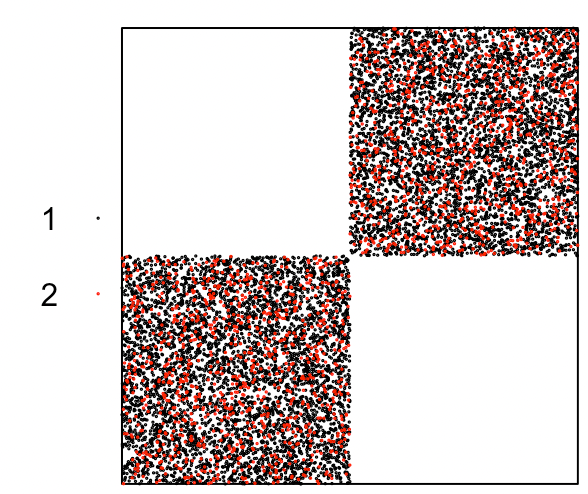
\includegraphics[width=8.17in]{Figures/Package Figs/Simulated_Data}

To see what each of the parameters do for this function, it's probably best to directly read the documentation. Here, I'll offer some advice on how to achieve a good tessellation/partition of the subspace. First, I'll start with a bad example: sigma (the bandwidth) is too small and the threshold is too high. Thus, the resulting intensity thresholded window has too much unnecessary white space, and the resulting windows are too''choppy.'' It also takes longer, and can lead to errors.

\begin{Shaded}
\begin{Highlighting}[]
\NormalTok{bad\_tessellation\_1 }\OtherTok{=} \FunctionTok{TessellateBiopsy}\NormalTok{(}\FunctionTok{PPPToTibble}\NormalTok{(ex\_biopsy\_excess),}
                                  \AttributeTok{sigma =} \DecValTok{1}\NormalTok{, }\AttributeTok{eps =} \DecValTok{15}\NormalTok{,}
                                  \AttributeTok{threshold =}\NormalTok{ (ex\_biopsy\_excess}\SpecialCharTok{$}\NormalTok{n)}\SpecialCharTok{/}
                                    \FunctionTok{area.owin}\NormalTok{(ex\_biopsy\_excess}\SpecialCharTok{$}\NormalTok{window),}
                                  \AttributeTok{clust.size =} \DecValTok{75}\NormalTok{,}
                                  \AttributeTok{max.clust.size =} \DecValTok{100}\NormalTok{)}
\end{Highlighting}
\end{Shaded}

Notice the ``checkerboard'' pattern of the tessellations:

\begin{Shaded}
\begin{Highlighting}[]
\FunctionTok{vis}\NormalTok{(bad\_tessellation\_1}\SpecialCharTok{$}\NormalTok{window)}
\end{Highlighting}
\end{Shaded}

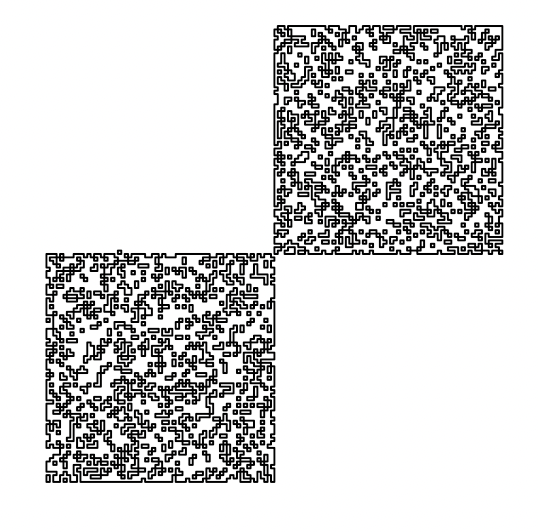
\includegraphics[width=7.47in]{Figures/Package Figs/bad_window}

This leads to poorly shaped tiles:

\begin{Shaded}
\begin{Highlighting}[]
\FunctionTok{vis}\NormalTok{(bad\_tessellation\_1}\SpecialCharTok{$}\NormalTok{tiles[[}\DecValTok{1}\NormalTok{]])}
\end{Highlighting}
\end{Shaded}

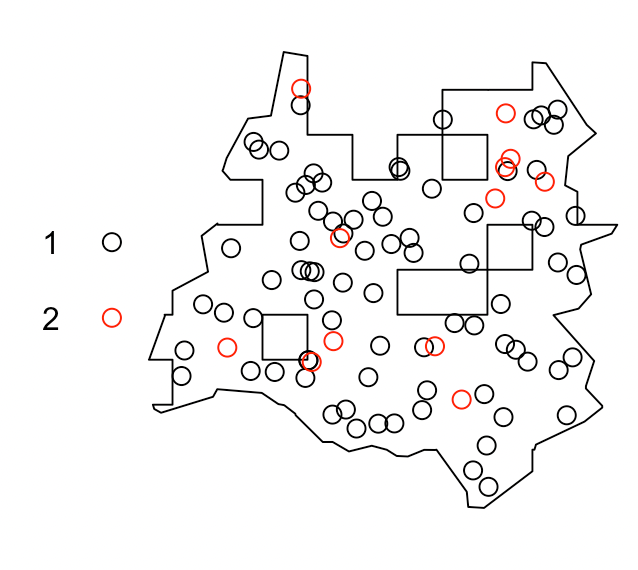
\includegraphics[width=8.86in]{Figures/Package Figs/bad_tile}

Let's try increasing the value of sigma. Note that all other parameters remain the same.

\begin{Shaded}
\begin{Highlighting}[]
\NormalTok{good\_tessellation }\OtherTok{=} \FunctionTok{TessellateBiopsy}\NormalTok{(}\FunctionTok{PPPToTibble}\NormalTok{(ex\_biopsy\_excess),}
                                 \AttributeTok{sigma =} \DecValTok{30}\NormalTok{, }\AttributeTok{eps =} \DecValTok{15}\NormalTok{,}
                                 \AttributeTok{threshold =}\NormalTok{ (ex\_biopsy\_excess}\SpecialCharTok{$}\NormalTok{n)}\SpecialCharTok{/}
                                   \FunctionTok{area.owin}\NormalTok{(ex\_biopsy\_excess}\SpecialCharTok{$}\NormalTok{window),}
                                 \AttributeTok{clust.size =} \DecValTok{75}\NormalTok{,}
                                 \AttributeTok{max.clust.size =} \DecValTok{100}\NormalTok{)}
\end{Highlighting}
\end{Shaded}

This looks much better:

\begin{Shaded}
\begin{Highlighting}[]
\FunctionTok{vis}\NormalTok{(good\_tessellation}\SpecialCharTok{$}\NormalTok{window)}
\end{Highlighting}
\end{Shaded}

\begin{Shaded}
\begin{Highlighting}[]
\NormalTok{knitr}\SpecialCharTok{::}\FunctionTok{include\_graphics}\NormalTok{(}\FunctionTok{here}\NormalTok{(}\StringTok{"Figures/Package Figs/good\_window.png"}\NormalTok{))}
\end{Highlighting}
\end{Shaded}

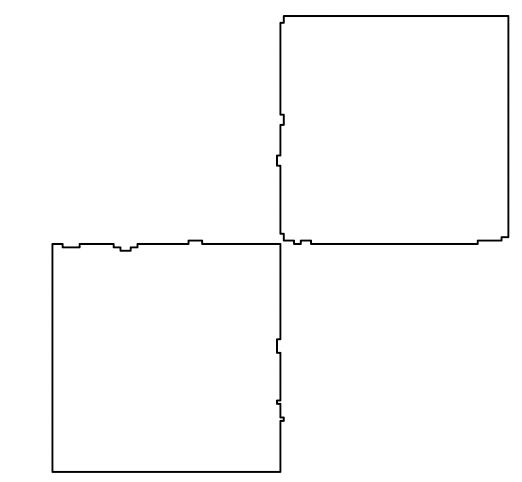
\includegraphics[width=7.25in]{Figures/Package Figs/good_window}

Ultimately, these are tuning parameters, and to find good values you may have to experiment a bit. The best advice I can offer is: start with a relatively large value of \texttt{sigma} (at least as large as \texttt{eps}), a relatively large value of \texttt{eps}, and a small \texttt{threshold}. Starting with a moderate \texttt{eps} is particularly important- if it's too small, the tessellation will not be computationally tractable. Once you have a working tessellation, reduce the values of sigma and eps as necessary, and increase the threshold as necessary. In my experience, the settings that work for one data set of a certain type will work for others; you should only need to go through this process once.

\hypertarget{interactive-visualization}{%
\section{Interactive Visualization}\label{interactive-visualization}}

Suppose you want to visualize all of the tiles all together, and a value associated with each tile. To do this, you can simply use the \texttt{PlotTessellation} function. First, we need a value to plot for each tile. In this case, I'll use the number of simulated tumor cells:

\begin{Shaded}
\begin{Highlighting}[]
\CommentTok{\# Result is a vector, each entry of which is the number of tumor cells}
\CommentTok{\# in the corresponding tile of the tessellation}
\NormalTok{bad\_tes\_n\_tum }\OtherTok{=} \FunctionTok{map\_dbl}\NormalTok{(bad\_tessellation\_1}\SpecialCharTok{$}\NormalTok{tiles, }\SpecialCharTok{\textasciitilde{}} \FunctionTok{sum}\NormalTok{(.x}\SpecialCharTok{$}\NormalTok{marks }\SpecialCharTok{==} \DecValTok{1}\NormalTok{))}
\NormalTok{good\_tes\_n\_tum }\OtherTok{=} \FunctionTok{map\_dbl}\NormalTok{(good\_tessellation}\SpecialCharTok{$}\NormalTok{tiles, }\SpecialCharTok{\textasciitilde{}} \FunctionTok{sum}\NormalTok{(.x}\SpecialCharTok{$}\NormalTok{marks }\SpecialCharTok{==} \DecValTok{1}\NormalTok{))}
\end{Highlighting}
\end{Shaded}

Then we pass both these things to the \texttt{PlotTessellation} function:

\begin{Shaded}
\begin{Highlighting}[]
\FunctionTok{PlotTessellation}\NormalTok{(bad\_tessellation\_1, bad\_tes\_n\_tum, }\StringTok{"\# Tumor Cells"}\NormalTok{)}
\end{Highlighting}
\end{Shaded}

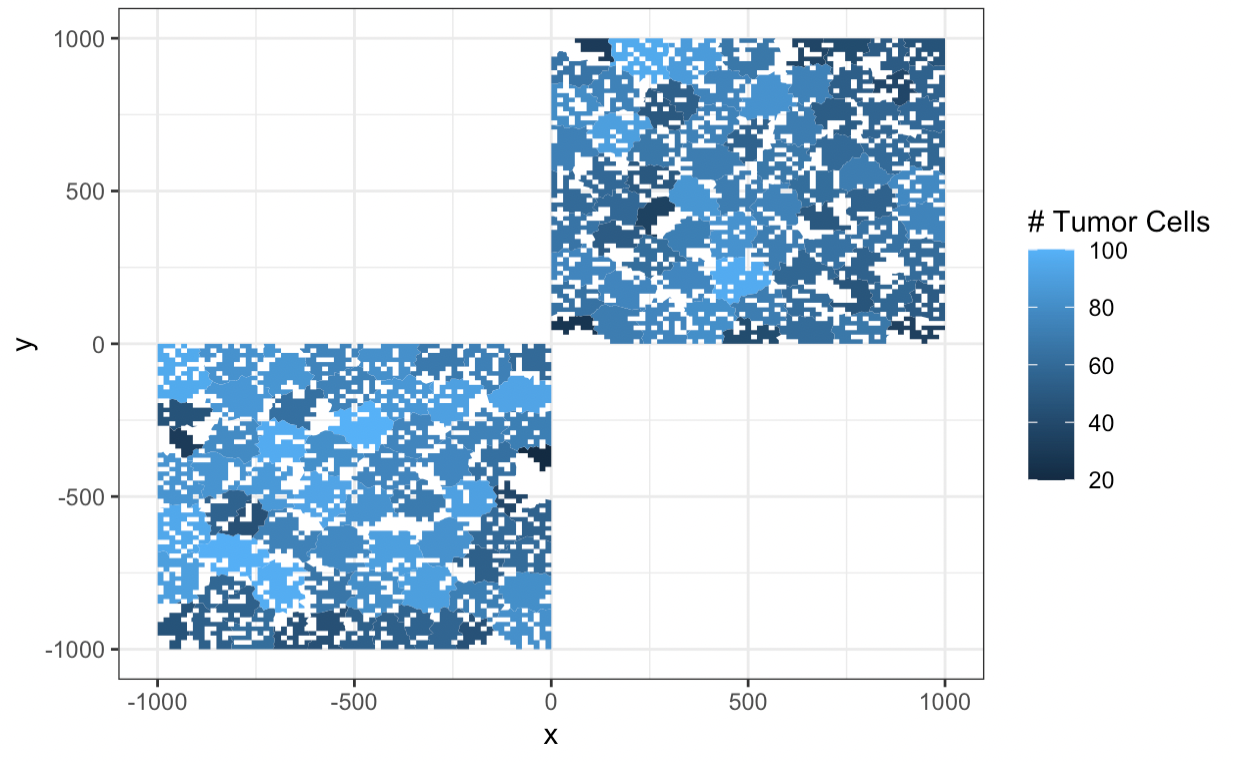
\includegraphics[width=17.14in]{Figures/Package Figs/bad_heatmap}

\begin{Shaded}
\begin{Highlighting}[]
\FunctionTok{PlotTessellation}\NormalTok{(good\_tessellation, good\_tes\_n\_tum, }\StringTok{"\# Tumor Cells"}\NormalTok{)}
\end{Highlighting}
\end{Shaded}

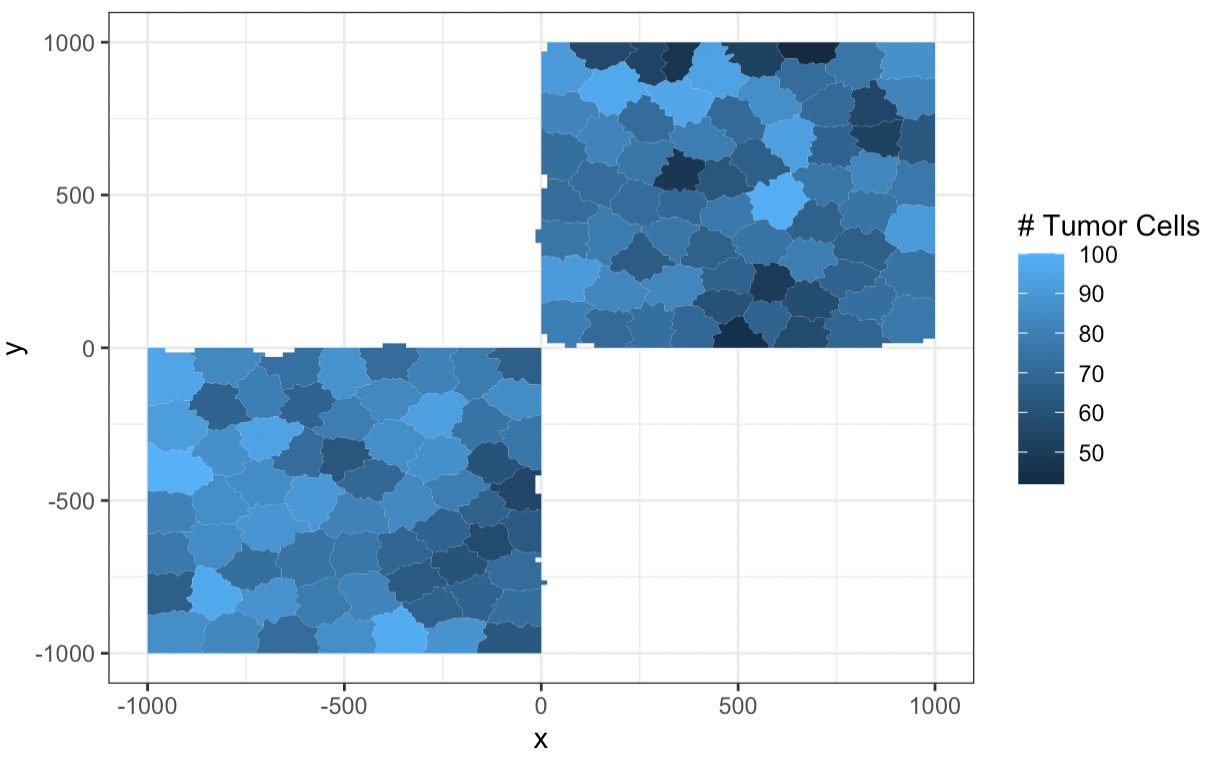
\includegraphics[width=16.89in]{Figures/Package Figs/good_heatmap}

However, there are clear limitations to this visualization method. What if you want to zoom in on a particular tile? Unfortunately, there's no easy way to do this in R. However, this can be easily accomplished in the companion web app, and the \texttt{ExportToVis} function. This function exports a tessellation as well as associated values so that they can be interactively visualized here: \url{https://nateosher.github.io/SPARTIN.html}.

In fact, unlike the static visualization above, it's fairly easy to switch between multiple tile level summaries. First, we create a list of all of the tile level values we want to summarize. Each list entry should have the same set of keys, each of which will be a value we're interested in. I'll keep it simple here and just use three: number of cells, number of tumor cells, and number of immune cells:

\begin{Shaded}
\begin{Highlighting}[]
\NormalTok{val\_list }\OtherTok{=} \FunctionTok{map}\NormalTok{(good\_tessellation}\SpecialCharTok{$}\NormalTok{tiles, }\ControlFlowTok{function}\NormalTok{(t)\{}
  \FunctionTok{list}\NormalTok{(}
    \AttributeTok{Cells =}\NormalTok{ t}\SpecialCharTok{$}\NormalTok{n,}
    \AttributeTok{Tumor =} \FunctionTok{sum}\NormalTok{(t}\SpecialCharTok{$}\NormalTok{marks }\SpecialCharTok{==} \DecValTok{1}\NormalTok{),}
    \AttributeTok{Immune =} \FunctionTok{sum}\NormalTok{(t}\SpecialCharTok{$}\NormalTok{marks }\SpecialCharTok{==} \DecValTok{2}\NormalTok{)}
\NormalTok{  )}
\NormalTok{\})}
\end{Highlighting}
\end{Shaded}

Then we export it. This command actually writes a \texttt{.json} file to the provided path:

\begin{Shaded}
\begin{Highlighting}[]
\FunctionTok{ExportToVis}\NormalTok{(good\_tessellation, val\_list, }\StringTok{"path/where/you/want/output"}\NormalTok{)}
\end{Highlighting}
\end{Shaded}

If you upload the resulting \texttt{.json} file to the visualization application, it will let you more easily examine multiple measures on the same biopsy, and zoom in on specific tiles to see the configuration of points.

  \bibliography{bibliography.bib}

\end{document}
